\documentclass[11pt]{article}

\usepackage[margin=1in]{geometry}
\usepackage{amsmath,amssymb,amsthm}
\usepackage{graphicx}
\usepackage{booktabs}
\usepackage{natbib}
\usepackage{hyperref}
\usepackage{xcolor}
\usepackage{titlesec}

\hypersetup{colorlinks=true, linkcolor=black, citecolor=blue!55!black,
            urlcolor=blue!55!black}
\graphicspath{{../figures/}}
\bibliographystyle{apalike}

\newtheorem{proposition}{Proposition}
\newtheorem{corollary}[proposition]{Corollary}

% Auto-generated by make_numbers.py -- do not edit by hand.
% Re-run `python3 make_numbers.py` after any phase is re-run.

\newcommand{\baselineCheckGain}{8.3}
\newcommand{\bayesAccCorr}{0.83}
\newcommand{\bayesAccHarm}{1.2}
\newcommand{\bayesAccMeanK}{2.00}
\newcommand{\bayesAccMeanP}{0.79}
\newcommand{\bayesAccMeanQ}{0.30}
\newcommand{\bayesAccdHlam}{1.45}
\newcommand{\bayesAccdHp}{0.77}
\newcommand{\bayesEpisodes}{2000}
\newcommand{\bayesFixCorr}{0.67}
\newcommand{\bayesFixHarm}{0.0}
\newcommand{\bayesFixKref}{6}
\newcommand{\bayesFixMeanK}{6.00}
\newcommand{\bayesFixMeanP}{0.50}
\newcommand{\bayesFixMeanQ}{0.11}
\newcommand{\bayesFixSdLamRatio}{151}
\newcommand{\bayesFixSdPRatio}{0.63}
\newcommand{\bayesFixdHlam}{4.80}
\newcommand{\bayesFixdHp}{-0.58}
\newcommand{\bayesFreeCorr}{0.84}
\newcommand{\bayesFreeHarm}{1.7}
\newcommand{\bayesFreeKref}{2}
\newcommand{\bayesFreeMeanK}{1.99}
\newcommand{\bayesFreeMeanP}{0.48}
\newcommand{\bayesFreeMeanQ}{0.08}
\newcommand{\bayesFreeSdLamRatio}{42}
\newcommand{\bayesFreeSdPRatio}{0.52}
\newcommand{\bayesFreedHlam}{3.35}
\newcommand{\bayesFreedHp}{-0.81}
\newcommand{\bayesVarCorr}{0.40}
\newcommand{\bayesVarHarm}{9.3}
\newcommand{\bayesVarKref}{3}
\newcommand{\bayesVarMeanK}{1.51}
\newcommand{\bayesVarMeanP}{0.77}
\newcommand{\bayesVarMeanQ}{0.29}
\newcommand{\bayesVarSdLamRatio}{17}
\newcommand{\bayesVarSdPRatio}{2.73}
\newcommand{\bayesVardHlam}{3.55}
\newcommand{\bayesVardHp}{0.81}
\newcommand{\bestDiversifiedGain}{8.6}
\newcommand{\calibChecker}{0.104}
\newcommand{\calibCheckerDown}{0.107}
\newcommand{\calibCurious}{0.113}
\newcommand{\calibCuriousDown}{0.169}
\newcommand{\calibLocked}{0.103}
\newcommand{\calibLockedDown}{0.172}
\newcommand{\calibQuota}{0.100}
\newcommand{\calibQuotaDown}{0.115}
\newcommand{\detBestTwoPoint}{5.68}
\newcommand{\detGraded}{4.96}
\newcommand{\detJittered}{-1.58}
\newcommand{\durFree}{0.35}
\newcommand{\durVariable}{0.07}
\newcommand{\erpAfterShiftP}{0.57}
\newcommand{\erpNaiveShiftP}{0.000}
\newcommand{\erpRiskDuring}{0.275}
\newcommand{\freeRiskDuring}{0.026}
\newcommand{\kappaCorrErr}{0.734}
\newcommand{\kappaCorrK}{0.988}
\newcommand{\kappaMax}{4.0}
\newcommand{\kappaMaxEarlyK}{9.8}
\newcommand{\kappaMaxErrP}{0.42}
\newcommand{\kappaMaxK}{4.10}
\newcommand{\kappaMaxLateK}{2.6}
\newcommand{\kappaZeroEarlyK}{4.2}
\newcommand{\kappaZeroErrP}{0.30}
\newcommand{\kappaZeroK}{1.96}
\newcommand{\kappaZeroLateK}{2.0}
\newcommand{\lockedGain}{2.1}
\newcommand{\loopChecker}{0.48}
\newcommand{\loopCurious}{0.38}
\newcommand{\loopLocked}{0.36}
\newcommand{\loopQuota}{0.38}
\newcommand{\nHypSupported}{11}
\newcommand{\nHypTotal}{11}
\newcommand{\nSingularPolicies}{4}
\newcommand{\phaseBestErr}{0.084}
\newcommand{\phaseBestK}{3}
\newcommand{\phaseCorrCostErrHigh}{-0.01}
\newcommand{\phaseCorrCostK}{0.86}
\newcommand{\phaseCorrDoubtErr}{-0.72}
\newcommand{\phaseErrAtZeroK}{0.70}
\newcommand{\phaseErrHighK}{0.31}
\newcommand{\phaseHarmAtBestK}{0.3}
\newcommand{\phaseHarmAtZeroK}{29.7}
\newcommand{\phaseHighDoubtErr}{0.50}
\newcommand{\phaseHighDoubtK}{1.97}
\newcommand{\phaseLowDoubtErr}{0.05}
\newcommand{\phaseLowDoubtK}{1.90}
\newcommand{\phaseWorstHighK}{6}
\newcommand{\postErpK}{2.98}
\newcommand{\postFreeQ}{0.07}
\newcommand{\postKtreated}{2.98}
\newcommand{\postKuntreated}{1.97}
\newcommand{\postVarQ}{0.27}
\newcommand{\preMeanK}{1.87}
\newcommand{\preMeanP}{0.28}
\newcommand{\preMeanQ}{0.10}
\newcommand{\preZq}{5.9}
\newcommand{\reassuranceGain}{2.3}
\newcommand{\reassuranceState}{0.021}
\newcommand{\seBestTwoPoint}{0.054}
\newcommand{\seJittered}{2.90}
\newcommand{\stepCheckerHalve}{847}
\newcommand{\stepCheckerK}{1.51}
\newcommand{\stepCheckerKhaz}{6.4}
\newcommand{\stepCheckerP}{0.66}
\newcommand{\stepCheckerQ}{0.027}
\newcommand{\stepCuriousHalve}{219}
\newcommand{\stepCuriousK}{0.04}
\newcommand{\stepCuriousKhaz}{5.9}
\newcommand{\stepCuriousP}{0.34}
\newcommand{\stepCuriousQ}{0.005}
\newcommand{\stepLockedHalve}{1153}
\newcommand{\stepLockedK}{2.79}
\newcommand{\stepLockedKhaz}{6.2}
\newcommand{\stepLockedP}{0.80}
\newcommand{\stepLockedQ}{0.323}
\newcommand{\stepQuotaHalve}{794}
\newcommand{\stepQuotaK}{1.24}
\newcommand{\stepQuotaKhaz}{4.7}
\newcommand{\stepQuotaP}{0.70}
\newcommand{\stepQuotaQ}{0.026}
\newcommand{\sweepBestK}{3}
\newcommand{\sweepBestdHp}{0.89}
\newcommand{\sweepCorrAtZero}{0.000}
\newcommand{\sweepKmax}{10}
\newcommand{\sweepMaxCorr}{0.88}
\newcommand{\sweepTaildHp}{0.07}
\newcommand{\tauLoErrMax}{0.13}
\newcommand{\tauLoErrZero}{0.26}
\newcommand{\tauLoHarmMax}{1.7}
\newcommand{\tauLoHarmZero}{1.0}
\newcommand{\tauLoKMax}{2.30}
\newcommand{\tauLoKZero}{2.17}
\newcommand{\tauLoMeanPMax}{0.67}
\newcommand{\tauLoMeanPZero}{0.54}
\newcommand{\tauLoVarMax}{0.123}
\newcommand{\tauLoVarZero}{0.118}
\newcommand{\tauMax}{300}
\newcommand{\tauMaxErr}{0.17}
\newcommand{\tauZeroErr}{0.29}
\newcommand{\txBaseHarm}{0.4}
\newcommand{\txBaseMeanP}{0.73}
\newcommand{\txErpHarm}{30.3}
\newcommand{\txErpHarmRate}{30}
\newcommand{\txErpMeanP}{0.67}
\newcommand{\txGradHarm}{12.3}
\newcommand{\txGradMeanP}{0.73}
\newcommand{\txLockHarm}{1.4}
\newcommand{\txLockMeanP}{0.37}
\newcommand{\txReaHarm}{1.7}
\newcommand{\txReaMeanP}{0.41}
\newcommand{\txVarHarm}{9.6}
\newcommand{\txVarMeanP}{0.71}
\newcommand{\uncCorrConcK}{0.31}
\newcommand{\uncHiConc}{200}
\newcommand{\uncHiErr}{0.35}
\newcommand{\uncHiK}{3.55}
\newcommand{\uncHiZ}{11.6}
\newcommand{\uncLoConc}{2}
\newcommand{\uncLoErr}{0.15}
\newcommand{\uncLoK}{1.97}
\newcommand{\uncLoZ}{0.7}
\newcommand{\variableGain}{7.1}
\newcommand{\vmBestDesign}{uniform 0..6}
\newcommand{\vmBestHarm}{5.5}
\newcommand{\vmBestSdP}{0.045}
\newcommand{\vmBestVarK}{4.0}
\newcommand{\vmCorr}{-0.94}
\newcommand{\vmFixedHarm}{0.2}
\newcommand{\vmFixedSdP}{0.147}
\newcommand{\vmSdRatio}{3.3}
\newcommand{\worldP}{0.80}
\newcommand{\worldQ}{0.30}
\newcommand{\zqFree}{5.8}
\newcommand{\zqVariable}{1.1}


\newcommand{\lamk}{\lambda_k}
\newcommand{\Ifisher}{\mathcal{I}}
\newcommand{\todo}[1]{\textcolor{red}{[#1]}}

\title{\textbf{Compulsions as Epistemic Traps:\\
Repetition Obscures Causal Control}}

\author{Dai Miyazaki\\
Graduate School of Humanities and Sociology, The University of Tokyo, Tokyo, Japan\\
Corresponding author: \texttt{dmyzk29@gmail.com}}

\date{September 4, 2026}

\begin{document}
\maketitle

\begin{abstract}
\noindent
Compulsive safety behaviour is commonly explained by biased beliefs about danger
or control, or by impaired learning. We identify a complementary mechanism that
requires neither deficit. In a hazard model, an episode starts in danger with
probability $q$, and each preventive repetition succeeds with probability $p$.
If an agent always repeats the action $k$ times, outcomes reveal only
$\lamk = q(1-p)^k$. The Fisher information is rank one, so $q$ and $p$ are
\emph{structurally non-identifiable} under any fixed-$k$ policy, regardless of
sample size. This theorem does not depend on a biased prior. Repetition removes
the variation needed to separate the two causes.
Simulations of exactly Bayesian agents show how this geometry matters: with an
initially pessimistic prior, a repetitive agent becomes precise about the observed
harm probability while remaining wrong about its causes; varying $k$ recovers both
parameters. Interventions restore information only when they create contrasts
between action counts. Thus, in this model, response prevention is informative
after a repetitive history but not from a naive start, while reassurance after
acting reduces current-state uncertainty and adds little causal information. At
matched mean exposure, the model predicts that trial-to-trial variability in
safety behaviour will be associated with more accurate knowledge of personal
efficacy. We present this as a computational mechanism and a set of falsifiable
human predictions, not as a complete account of OCD.
\end{abstract}

\section*{Author Summary}

People who repeatedly perform a safety action can learn that the immediate outcome is usually safe
without learning whether safety came from the world being safe or from their action. This study
formalises that problem. We model a person who faces danger with some probability and whose preventive
action sometimes works. If the person always repeats the action the same number of times, the observations
contain only one combined measure of danger and action success. No amount of additional experience can
separate the two causes. Computer simulations show that an ideally rational learner can therefore become
confident about what will happen while remaining uncertain, or becoming confidently wrong, about why.
Small, well-chosen changes in the number of repetitions restore the missing information; checks performed
after acting do not. The model makes a testable prediction for human research: among people with similar
average safety behaviour and symptom severity, greater trial-to-trial variation in safety behaviour should
be associated with more accurate knowledge of how effective their actions are. This mechanism does not by
itself explain every feature of compulsions, but it identifies a precise way in which protection can
prevent learning.

\vspace{1em}
\noindent\textbf{Keywords:} obsessive-compulsive disorder; structural
identifiability; Bayesian learning; safety behaviour; exposure and response
prevention.

\section{Introduction}

\subsection{A hundred checks, and still no answer}

Someone worries that they have left the door unlocked, so they go back and check.
The obvious account of what follows is that anxiety drives repetition: the more
frightened they are, the more they check. That account explains why they check.
It does not explain the thing that most needs explaining, which is why the
hundredth check leaves them no more certain than the first.

None of this is a new observation clinically. The cognitive theory of compulsive
checking \citep{rachman2002checking} already holds that checking maintains itself,
and a well-replicated experimental literature shows that repeated checking
degrades confidence in one's own memory rather than improving it
\citep{vandenhout2003repeated,abbasi2023checking}; in compulsivity, confidence can
come apart from performance altogether
\citep{vaghi2017compulsivity,seow2020transdiagnostic}. Our
contribution is not to notice the phenomenon but to say, exactly, what makes it
inevitable --- and the uncertainty we formalise is not confidence in a memory but
knowledge of a latent causal parameter.

Here is a different way to look at it. Each time they check, they remove the
comparison that would have told them something. If they never leave without
checking, they never find out whether the door would have been locked anyway.
They cannot separate ``the door was already locked'' from ``the door is locked
\emph{because} I checked''. Every check is safe and every check is uninformative
about the one thing they want to know, which is whether their own action is what
is keeping them safe. This paper turns that observation into a theorem.

\subsection{Two existing explanations, and a third}

Two computational accounts of compulsion are well developed.
\citet{rigoux2024beliefs} model a handwashing scenario as a partially observable
Markov decision process and show that a single belief distortion --- an
underestimation of the probability that one's preventive action succeeds ---
triggers and maintains compulsive behaviour and scales with its severity. On this
account the pathology sits in a \emph{belief}: the agent's point estimate of its
own efficacy is too low. \citet{sakai2022eligibility} locate the pathology
instead in a \emph{learning mechanism}: an imbalance between the memory traces
that assign credit to reinforcement and to punishment. Related accounts place it
in uncertainty about state transitions
\citep{fradkin2020searching,fradkin2020latent,prudon2021,sharp2023transition}, in
habitual avoidance \citep{gillan2014enhanced}, or in a failure to integrate
local evidence into a stable global belief. In the
clinical literature the corresponding idea is that safety behaviour preserves
threat beliefs by preventing their disconfirmation
\citep{lovibond2009safety,craske2014inhibitory}, and that low-cost avoidance
survives even after fear has been extinguished \citep{vervliet2015low}.

We propose a third possibility, orthogonal to both. Suppose the agent's belief
updating and credit assignment are exact. It can still remain ignorant of its
own efficacy for as long as it keeps behaving the same way, because its policy
decides which comparisons enter the data and a repetitive policy admits none.
We show this first as a theorem (Section~\ref{sec:theorem}) and then in a
controlled simulation that varies only the design (Fig.~\ref{fig:fig3}F). The
mechanism lies in the geometry of the evidence the learner's behaviour generates,
not necessarily in a learning deficit.

\citet{rigoux2024beliefs} state a related gap: their model does not describe how
beliefs about world contingencies are acquired, and its agent parameters are
static point estimates rather than time-varying posteriors. Our extension makes
that acquisition problem explicit and separates what follows from information
structure from what depends on belief or credit-assignment parameters.

\subsection{What is new}

\paragraph{A mathematical result.} Under a fixed repetition count, baseline
hazard and personal efficacy are non-identifiable, not merely difficult to
estimate. The terminal-outcome information matrix is rank one for every $k$ and
every interior $(q,p)$ (Proposition~\ref{prop:rank1}).

\paragraph{A mechanism independent of learner failure.} The result holds for an
ideal Bayesian learner, so it does not require impaired updating or credit
assignment. The simulations use a deliberately pessimistic initial prior; the
theorem itself is prior-independent. The claim is about the evidence generated
by a policy, not about how people with obsessive-compulsive disorder learn in
general.

\paragraph{A sharper account of response prevention.} Setting $k=0$ samples the
baseline hazard $q$ but supplies zero information about $p$. Response prevention
is informative about efficacy only when it is combined with episodes at a
different action count. What restores identifiability is policy variation, not
the absence of safety behaviour by itself.

\paragraph{A temporal dissociation.} State uncertainty and structural
uncertainty are distinct in the model. A reassurance-like probe after acting
reduces the former but barely changes the latter; the same probe before acting is
diagnostic about the latent causes.

\subsection{The general principle}

Knowing whether you control something requires having varied what you do and
compared the results. When the cost of failure is high, the behaviour that
minimises immediate risk suppresses exactly that variation. Safety can be locally
optimal and globally destructive of self-knowledge. This is not a claim about
obsessive-compulsive disorder alone; it is the same structure that appears as a
failure of persistent excitation in system identification, as self-confirming
equilibrium in economics \citep{fudenberg1993selfconfirming}, as the selective
labels problem in machine learning \citep{lakkaraju2017selective}, and as
algorithmic feedback loops in recommender systems
\citep{chaney2018algorithmic}. We develop the case in the setting of compulsion
because that is where it has a face, and generalise in the Discussion.
Figure~\ref{fig:fig1} states the shift in one picture.

\begin{figure}[t]\centering
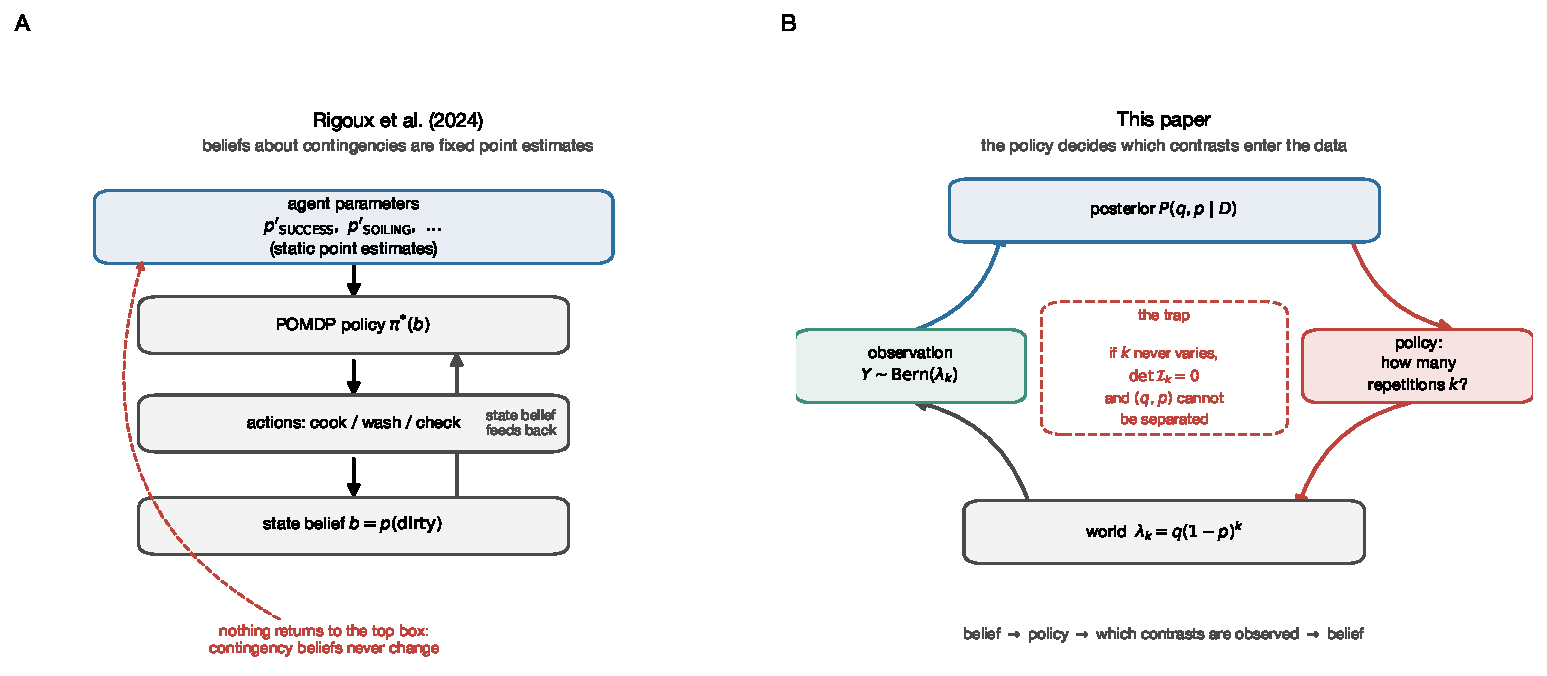
\includegraphics[width=\textwidth]{fig1_concept.pdf}
\caption{\textbf{From fixed beliefs to a closed causal-learning loop.}
(A) In \citet{rigoux2024beliefs} the agent's beliefs about world contingencies are
static point estimates: the state belief is updated every trial, but nothing ever
returns to the box at the top, so the model cannot say how those contingency
beliefs were acquired or why they are not corrected. (B) Here they are a
posterior, and the posterior chooses the policy, and the policy decides which
contrasts enter the data. When the number of repetitions $k$ never varies, the
resulting design is rank one and $(q,p)$ cannot be separated however long the loop
runs.}
\label{fig:fig1}
\end{figure}

\section{Model}

\subsection{The Rigoux baseline}
\label{sec:baseline}

We first reproduce the model we extend. \citet{rigoux2024beliefs} consider a
cooking scenario with states $S=\{\text{clean},\text{dirty}\}$ and actions
$A=\{\text{cook},\text{wash},\text{check}\}$. Cooking with clean hands is
rewarding and may soil them with probability $p_{\mathrm{SOILING}}$; cooking with
dirty hands is costly; washing cleans dirty hands with probability
$p_{\mathrm{SUCCESS}}$; checking changes nothing but returns a noisy observation
of the state. The agent cannot observe the state and acts on a belief
$b = P(\text{dirty})$, updated by Bayes' rule, in the standard partially
observable Markov decision framework \citep{kaelbling1998planning}. Crucially, each simulated
individual carries two parameter sets: objective \emph{world} parameters that
generate transitions and observations, and subjective \emph{agent} parameters
that generate the policy --- both, in the original, static point estimates.

Because the state space has two elements, the belief simplex is the interval
$[0,1]$ and the value function can be obtained by discounted value iteration on a
fine belief grid with linear interpolation; we use this in place of the
incremental-pruning solver of the original.

\subsection{Episodes, and the composite the agent can see}

For the identifiability analysis we work with a reduced description of one
symptom-provoking episode, which we take to be the essential structure of the
Rigoux scenario:
\begin{enumerate}\itemsep2pt
\item the episode begins in the hazardous state with probability $q$ (in the
      original, $p_{\mathrm{SOILING}}$);
\item the agent performs $k$ preventive repetitions, each removing the hazard
      with probability $p$ (in the original, $p_{\mathrm{SUCCESS}}$);
\item the agent commits to the consequential action; harm occurs if and only if
      the hazard is still present.
\end{enumerate}
Writing $Y=1$ for harm,
\begin{equation}
Y \sim \mathrm{Bernoulli}(\lamk), \qquad \lamk = q(1-p)^{k}.
\label{eq:lambda}
\end{equation}
Everything the agent can observe about $(q,p)$ from outcomes passes through the
scalar $\lamk$. That is the whole of the problem.

\subsection{The rank-one theorem}
\label{sec:theorem}

\begin{proposition}[Fixed-$k$ designs are singular]
\label{prop:rank1}
Let $\theta=(q,p)\in(0,1)^2$ and let $Y\sim\mathrm{Bernoulli}(\lamk)$ with $\lamk$
as in \eqref{eq:lambda} for a fixed $k\ge 0$. Then the Fisher information of one
observation,
\begin{equation}
\Ifisher_k(\theta) \;=\;
\frac{\nabla_\theta \lamk \, \nabla_\theta \lamk^{\top}}{\lamk(1-\lamk)},
\qquad
\nabla_\theta \lamk =
\begin{bmatrix} (1-p)^{k} \\[2pt] -kq(1-p)^{k-1}\end{bmatrix},
\label{eq:fisher}
\end{equation}
has rank one and $\det \Ifisher_k(\theta) = 0$ identically. Consequently $(q,p)$
is not locally identifiable from any number of episodes run at a single $k$.
\end{proposition}

\begin{proof}
$\Ifisher_k$ is a scalar multiple of the outer product of a single vector with
itself, hence has rank at most one; it is exactly one at interior $\theta$ since
$\nabla_\theta\lamk \neq 0$. A $2\times2$ matrix of rank one has zero
determinant. Independent observations add information, so the total information
from $n$ episodes at the same $k$ is $n\Ifisher_k$, still singular. The explicit
ridge in Corollary~\ref{cor:ridge} establishes the failure of local
identifiability directly; the Fisher calculation records its local rank
deficiency. This is the distinction between a parameterisation that is not
identified and an estimator that is merely imprecise.
\end{proof}

The derivation is verified symbolically in \texttt{phase1\_nonidentifiability.py}
and machine-checked in the test suite for a range of parameter values.

\begin{corollary}[The trap has a direction]
\label{cor:ridge}
The null direction of $\Ifisher_k$ is tangent to the iso-likelihood curve
$q = \lambda_0 (1-p)^{-k}$, whose slope is
\begin{equation}
\frac{dq}{dp}\bigg|_{\lamk\ \mathrm{const}} = \frac{kq}{1-p} \;\ge\; 0 .
\label{eq:slope}
\end{equation}
The residual dependence between $q$ and $p$ is therefore \emph{positive}, and the
ridge steepens with $k$: an agent that repeats more cannot tell a dangerous world
it controls from a safe world it does not.
\end{corollary}

A caution about reading Corollary~\ref{cor:ridge} empirically. It is a statement
about the \emph{likelihood}, and the posterior correlation it induces also depends
on how much likelihood there is to speak of. As $k$ grows, $\lamk \to 0$ and
outcomes stop being surprising, so the posterior reverts towards the prior and the
measured coupling falls back to zero. Non-identifiability and uninformativeness
are two distinct failures --- at small $k$ the agent learns a combination it
cannot decompose, at large $k$ it learns nothing at all --- and the simulations in
Section~3.3 show both, with a maximum in between.

\begin{proposition}[Two conditions suffice, and one does not]
\label{prop:two}
For $k_1 \neq k_2$ with $\lambda_{k_1},\lambda_{k_2}$ known,
\begin{equation}
\frac{\lambda_{k_1}}{\lambda_{k_2}} = (1-p)^{k_1-k_2}
\;\Longrightarrow\;
p = 1 - \left(\frac{\lambda_{k_1}}{\lambda_{k_2}}\right)^{1/(k_1-k_2)},
\quad
q = \lambda_{k_1}(1-p)^{-k_1},
\label{eq:recovery}
\end{equation}
so a policy with support on two distinct values of $k$ point-identifies
$(q,p)$. In particular, at $k=0$ the likelihood \eqref{eq:lambda} does not depend
on $p$; response prevention alone identifies $q$ exactly and carries no
information whatsoever about $p$.
\end{proposition}

For a policy $\pi$ over repetition counts, information adds as
$\Ifisher_\pi = n\sum_k \pi(k)\,\Ifisher_k$, and it is the \emph{support} of
$\pi$, not its mean, that determines rank. In control-theoretic terms, a
compulsive policy is a failure of persistent excitation: the agent drives the
system in a way that is safe locally and uninformative about the system's causal
parameters. The framing descends from \citet{bellman1970structural}, who asked
what experiments determine internal structure from input--output measurement.

\subsection{The Bayesian agent}

We replace the original's static point estimates with a joint posterior over
$(q,p)$ on a $101\times101$ midpoint grid, updated exactly. Priors are
independent Beta distributions; grid inference rather than MCMC keeps every
simulation deterministic given a seed. The agent's subjective expected cost of
committing to $k$ repetitions is
\begin{equation}
C(k) \;=\; c_{\mathrm{harm}}\Big(\mathbb{E}[\lamk] + \kappa\,\mathrm{SD}[\lamk]\Big)
        \;+\; c_{\mathrm{wash}}\,k ,
\label{eq:cost}
\end{equation}
and it selects $k$ by a softmax on $U(k) = -C(k) + \tau\,\mathrm{EIG}(k)$, where
$\mathrm{EIG}(k) = I\big((q,p);Y \mid k, D\big)$ is the expected information gain
of \citet{lindley1956measure} and \citet{chaloner1995bayesian}. The two extra
parameters have interpretations we use rather than hide: $\kappa>0$ is
intolerance of uncertainty --- the agent pays for the \emph{variance} of the
hazard, not only its mean --- and $\tau>0$ is a willingness to pay for causal
knowledge. The baseline agent has $\kappa=\tau=0$ and is a pure harm minimiser.

We distinguish two kinds of uncertainty throughout. \emph{State} uncertainty is
the entropy of the agent's belief that the hazard is present in the current
episode at the moment of commitment. \emph{Structural} uncertainty is the entropy
of the posterior over $(q,p)$. Reassurance and exposure act on these differently,
which is the content of Section~\ref{sec:interventions}.

Finally, we score knowledge by the log posterior density at the true parameter,
$\log P(q^\ast,p^\ast \mid D)$, not by entropy alone. Entropy rewards confidence,
and one of our findings is precisely that an untreated agent becomes confident
and wrong.

\section{Results}

\subsection{Replication of the point-belief model}

Simulating $\repNagents$ agents across $\repNworlds$ worlds in which repeated
washing or checking is not optimal (Fig.~\ref{fig:figS1}), compulsive agents
underestimate the
effectiveness of their preventive action relative to non-compulsive agents
($\Delta p_{\mathrm{SUCCESS}} = \repDeltaPsuccessComp$ vs
$\repDeltaPsuccessNon$; Cohen's $d = \repDsuccess$, cluster bootstrap over worlds
$p \repPsuccessP$), while beliefs about perception do not separate the groups
($d = \repDdetectDirty$ for $p_{\mathrm{DETECT,DIRTY}}$). We depart from the
original in two respects, both stated rather than smoothed over. First, our
world-selection criterion favours worlds in which washing is effective (mean
world $p_{\mathrm{SUCCESS}} = \repWorldPsuccess$), so both groups show negative
$\Delta p_{\mathrm{SUCCESS}}$ on average and it is the between-group contrast
that carries the result. Second, unlike the original we find group differences of
comparable or larger size in cost parameters ($d = \repDsick$ for
$\mathrm{cost}_{\mathrm{SICKNESS}}$, $d = \repDcheck$ for
$\mathrm{cost}_{\mathrm{CHECK}}$), which we attribute to our grid value-iteration
solver and world sample rather than to a substantive disagreement.
This makes Phase 0 a partial replication rather than an exact reproduction; the
claim should be checked against the authors' released solver before submission if
that code can be run in the same environment.

The severity gradient replicates. Among compulsive agents, greater underestimation
of efficacy predicts longer compulsive episodes (Spearman
$\rho = \repRhoMaxLen$ for the longest episode, $\repRhoMeanLen$ for the mean, and
$\repRhoWithinWorld$ within worlds) and a larger fraction of non-consequential
actions ($\rho = \repRhoFracNoncook$). The \emph{number} of episodes moves the
other way ($\rho = \repRhoNepisodes$), as it must when episodes get longer. We
report rank correlations because episode lengths are heavy-tailed and Pearson
correlations here are dominated by a handful of very long runs.

\begin{figure}[t]\centering
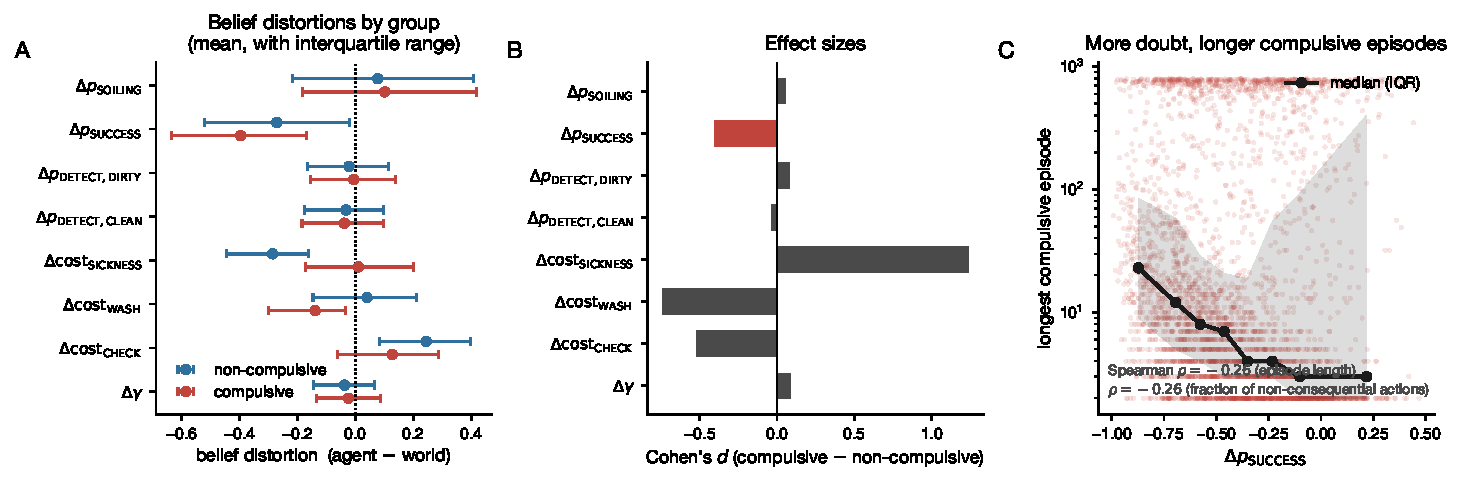
\includegraphics[width=\textwidth]{fig_S1_replication.pdf}
\caption{\textbf{Supplementary: replication of the point-belief model.}
$\repNagents$ agents across $\repNworlds$ worlds in which repeated washing or
checking is not optimal. (A) Belief distortions by group (mean, interquartile
range). (B) Effect sizes; $\Delta p_{\mathrm{SUCCESS}}$ in red. (C) Among
compulsive agents, greater underestimation of efficacy predicts longer compulsive
episodes; medians with interquartile range, quantified by Spearman rank
correlation. Two departures from the original are discussed in the text: our world
selection favours worlds in which washing is effective, and we find group
differences in cost parameters that the original did not.}
\label{fig:figS1}
\end{figure}

\subsection{Non-identifiability is a theorem, not a finding}

Figure~\ref{fig:fig2} makes Proposition~\ref{prop:rank1} visible. At fixed $k$,
the log-likelihood surface over $(q,p)$ is a ridge rather than a peak (panel A),
and by Corollary~\ref{cor:ridge} the ridge steepens with $k$ (panel B), so
$\det\Ifisher_k$ vanishes for every $k$ (panel C). Comparing candidate policies
at matched episode counts (panel D), all $\nSingularPolicies$ single-$k$ policies
are singular, while every policy with support on two or more values of $k$ is
not. The ordering among the non-singular policies is instructive: the best design
is not the most extreme but the most balanced. A policy alternating $k\in\{0,1\}$
attains $\log_{10}\det\Ifisher_\pi = \detBestTwoPoint$; spreading uniformly over
$k\in\{0,\dots,6\}$ attains only $\detGraded$, because episodes at large $k$
almost never produce an informative outcome. A ``compulsive but jittered'' policy
on $k\in\{5,6,7\}$ is formally non-singular yet practically useless
($\detJittered$; standard error on $p$ of $\seJittered$ versus $\seBestTwoPoint$
for $k\in\{0,1\}$). Variation matters, but variation \emph{where outcomes still
happen}.

\begin{figure}[t]\centering
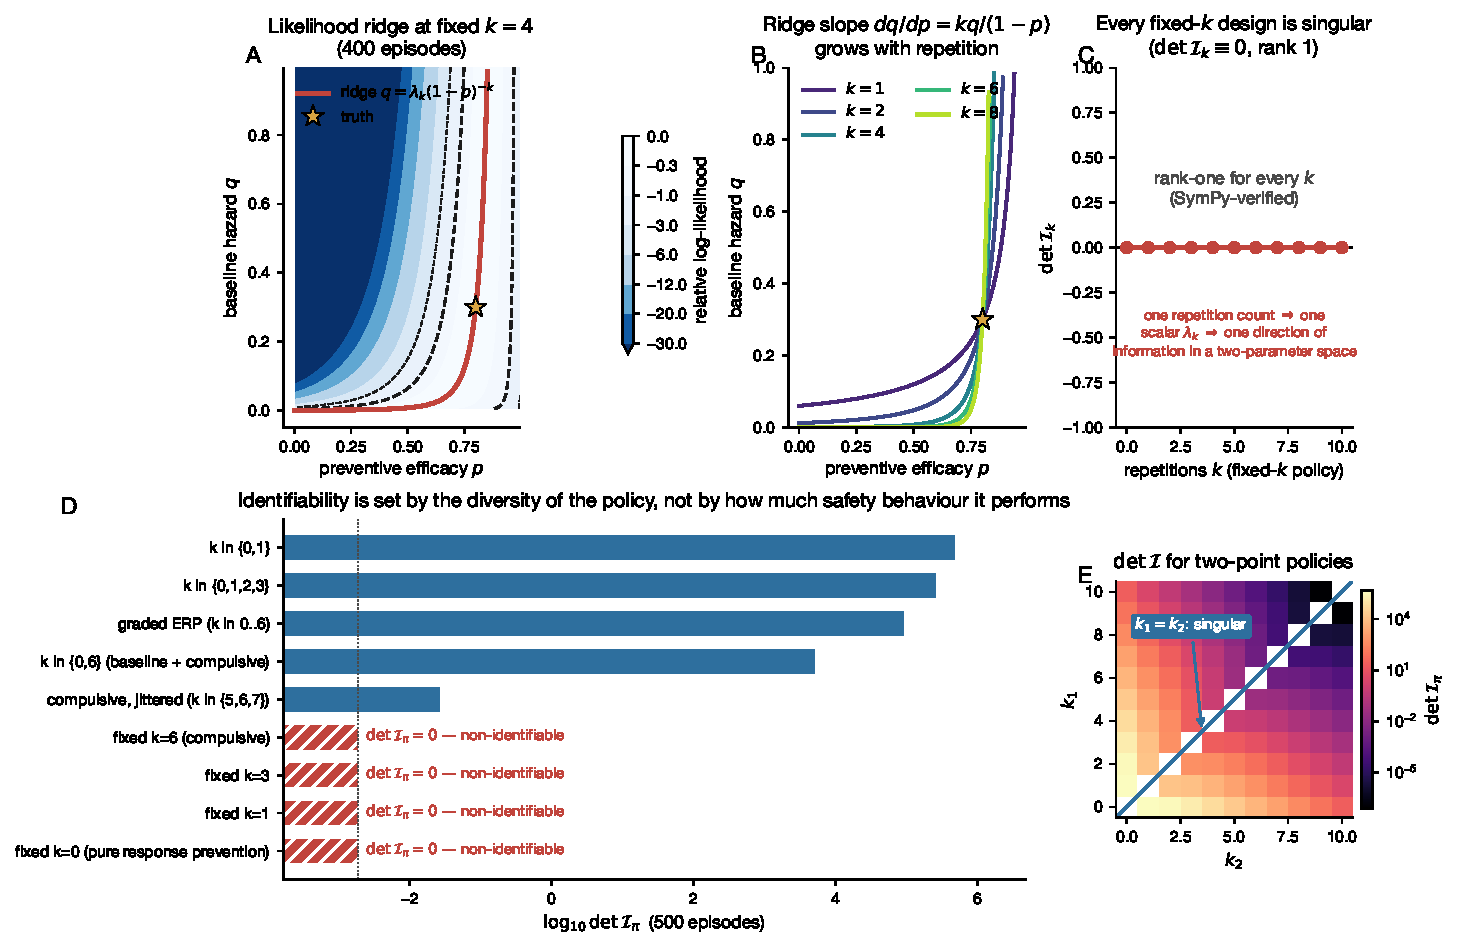
\includegraphics[width=\textwidth]{fig2_nonidentifiability.pdf}
\caption{\textbf{Structural non-identifiability under a repetitive policy.}
(A) Log-likelihood over $(q,p)$ from 400 episodes at fixed $k=4$: a ridge, not a
peak. (B) The ridge $q=\lambda_k(1-p)^{-k}$ steepens with $k$
(Corollary~\ref{cor:ridge}). (C) $\det\Ifisher_k \equiv 0$ for every $k$,
verified symbolically. (D) Identifiability of candidate policies at 500 episodes;
every single-$k$ policy is singular. (E) $\det\Ifisher$ for every two-point
policy $\{k_1,k_2\}$; the diagonal $k_1=k_2$ is the singular set.}
\label{fig:fig2}
\end{figure}

\subsection{What a repetitive learner ends up knowing}

Figure~\ref{fig:fig3} follows exactly-Bayesian agents for $\bayesEpisodes$
episodes in a world with $q^\ast=\worldQ$ and $p^\ast=\worldP$. An agent with a
severe initial doubt about its efficacy that holds its repetition count fixed
ends at $\mathbb{E}[p\mid D] = \bayesFixMeanP$ and
$\mathbb{E}[q\mid D] = \bayesFixMeanQ$, with a posterior correlation of
$\bayesFixCorr$ between the two, and it experiences harm on $\bayesFixHarm\%$ of
episodes. An otherwise identical agent whose policy draws $k$ from
$\{0,1,2,3\}$ ends at $\mathbb{E}[p\mid D] = \bayesVarMeanP$ and
$\mathbb{E}[q\mid D] = \bayesVarMeanQ$ --- both close to the truth --- at the cost
of harm on $\bayesVarHarm\%$ of episodes.

The signature of the trap is the contrast between what is learned and what is
not. The repetitive agent gains $\bayesFixdHlam$ nats about the observable
composite $\lamk$ and $\bayesFixdHp$ nats about $p$ (Fig.~\ref{fig:fig3}C). The
same contrast in scale-free terms is starker still: relative to its prior, the
agent's posterior standard deviation for the observable
$\lambda_{\bayesFixKref}$ shrinks by a factor of $\bayesFixSdLamRatio$, while its
uncertainty about $p$ does not shrink at all --- it \emph{grows}, by a factor of
$1/\bayesFixSdPRatio$, as the data push it off a prior that was narrow and wrong
onto a ridge that is broad. It can predict what will happen to it with great
precision while becoming \emph{less} sure why. The diversified agent shows the
opposite pattern: $\bayesVarSdLamRatio\times$ on the observable and
$\bayesVarSdPRatio\times$ on the parameter. (We report the ratios alongside the
entropies because the entropy of $\lamk$ is computed on a fixed $[0,1]$ bin grid
and saturates when $\lamk$ becomes very small, so the nats figure is a lower
bound on the information gained.) The repetitive agent's final posterior lies
along the analytic ridge (Fig.~\ref{fig:fig3}D); the diversified agent's sits at
the intersection of the ridges belonging to the different $k$ it used
(Fig.~\ref{fig:fig3}E).

Holding the prior fixed and varying only the design
(Fig.~\ref{fig:fig3}F) shows that information about one's own efficacy is
maximised at an intermediate and rather small number of repetitions
($k=\sweepBestK$; $\sweepBestdHp$ nats) and falls away at both ends: exactly zero
at $k=0$, where the likelihood does not depend on $p$, and $\sweepTaildHp$ nats
at $k=\sweepKmax$, where harm has become so rare that no outcome is surprising.
Posterior coupling between $q$ and $p$ behaves the same way, peaking at
$\sweepMaxCorr$ and vanishing at $k=0$ ($\sweepCorrAtZero$). The two ends of the
range are two different failures: at $k=0$ the agent learns a parameter that is
not the one it cares about; at large $k$ it learns nothing at all.

\begin{figure}[t]\centering
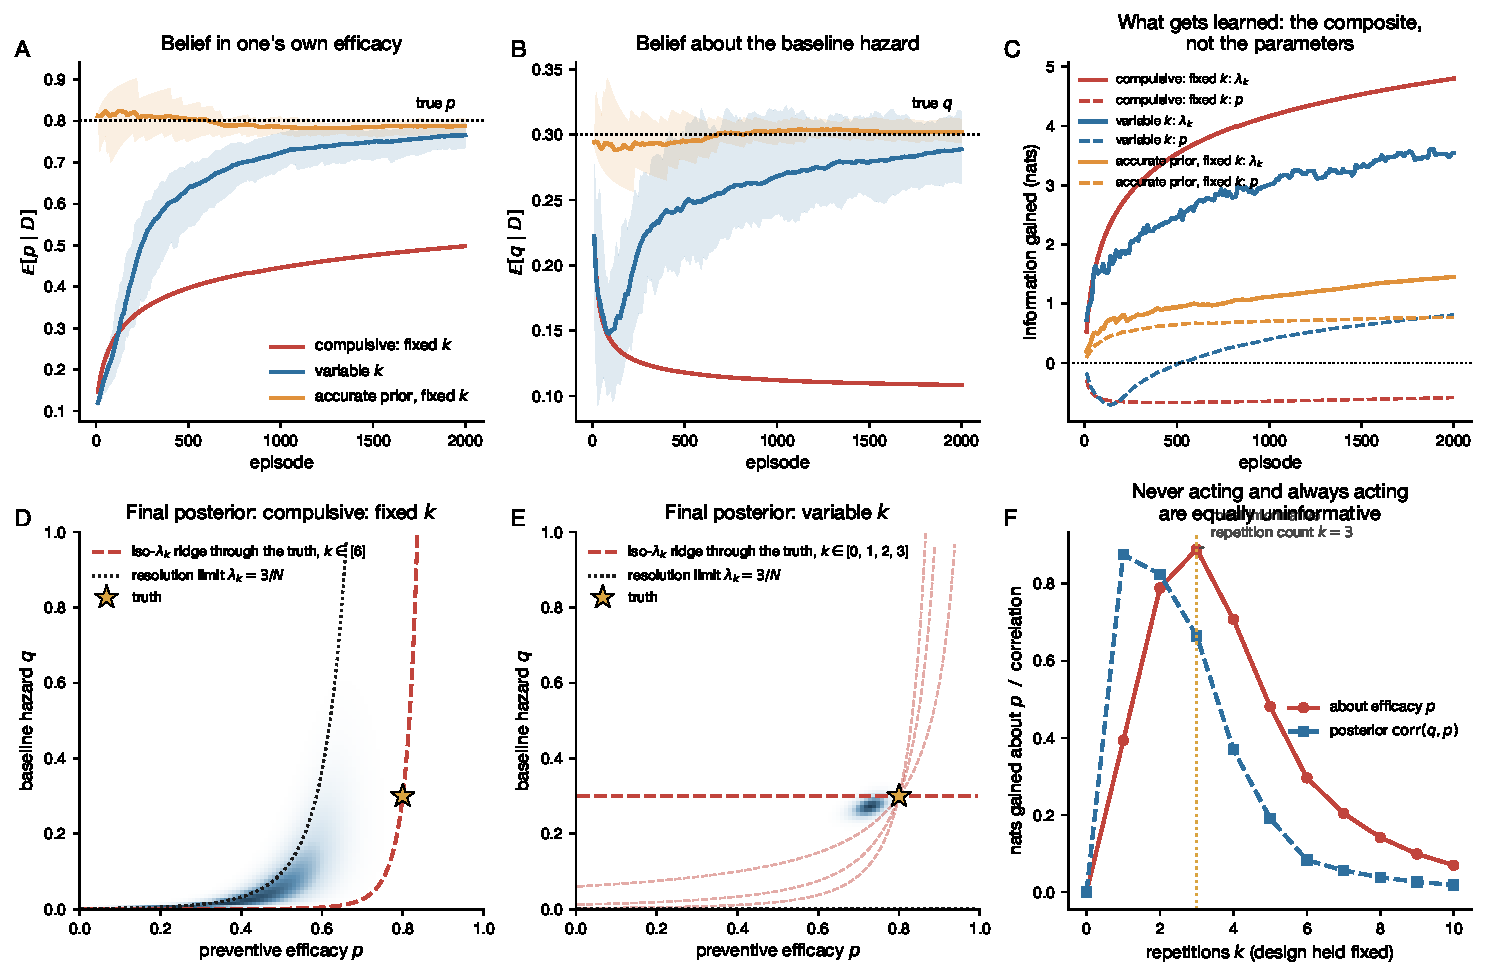
\includegraphics[width=\textwidth]{fig3_posterior_trajectories.pdf}
\caption{\textbf{What a repetitive learner ends up knowing.} (A,B) Posterior
means for efficacy and baseline hazard; shading is the 10--90th percentile across
agents. (C) Information gained about the observable composite $\lamk$ (solid)
versus the parameter $p$ (dashed). (D,E) Final joint posteriors with the analytic
iso-$\lamk$ ridges and the resolution limit $\lamk = 3/N$. (F) With the prior held
fixed and only the design varying, information about $p$ is maximised at a small
interior $k$.}
\label{fig:fig3}
\end{figure}

\subsection{Does the loop close? Uncertainty aversion}

A purely harm-minimising agent that begins in doubt does not remain
behaviourally compulsive forever. As its estimate of $p$ creeps up its repetition
count drifts down, from an early mean of $\kappaZeroEarlyK$ to $\kappaZeroLateK$,
even though its efficacy belief remains far from the truth
($|\mathbb{E}[p\mid D]-p^\ast| = \kappaZeroErrP$). In this model, then, the trap
is primarily epistemic: the belief stays wrong for thousands of episodes while
the behaviour partially normalises.

The natural candidate for the missing behavioural ingredient is intolerance of
uncertainty, and the model contains it as $\kappa$ in \eqref{eq:cost}: an agent
that pays for the \emph{variance} of the hazard as well as its mean. Sweeping
$\kappa$ has two effects, and we report both, including the one that does not go
our way. It raises the amount of safety behaviour monotonically (mean $k$ from
$\kappaZeroK$ at $\kappa=0$ to $\kappaMaxK$ at $\kappa=\kappaMax$;
$r = \kappaCorrK$) and it deepens the epistemic trap, with the residual error in
the efficacy belief rising from $\kappaZeroErrP$ to $\kappaMaxErrP$
($r = \kappaCorrErr$). It does \emph{not}, however, prevent behavioural decay
over $\bayesEpisodes$ episodes: even at $\kappa=\kappaMax$ the repetition count
falls from $\kappaMaxEarlyK$ early to $\kappaMaxLateK$ late.

We therefore state hypothesis H2 in the form the simulations support rather than
the form we set out to test. Uncertainty aversion strengthens the loop --- more
repetition, worse knowledge --- but a fully self-sustaining behavioural
compulsion is not produced by these two ingredients alone within this horizon.
What is produced, robustly, is a learner that is persistently and confidently
wrong about its own efficacy.

A post-hoc boundary check asks what happens if one more psychological ingredient
is added. In a responsibility-feedback policy, the subjective cost of harm is
multiplied by $1+\alpha R_t$, where $R_t$ is an exponentially weighted trace of
recent repetition. With no such feedback, the late/early repetition ratio is
$\respBasePersistence$ and the late repetition count is $\respBaseLateK$. The
first feedback strength that meets our behavioural-closure criterion is
$\alpha=\respClosedStrength$, with a late/early ratio of
$\respClosedPersistence$ and a late repetition count of $\respClosedLateK$; the
agent remains wrong about efficacy ($|\mathbb{E}[p]-p^\ast|=\respClosedErrP$)
and experiences harm on only $\respClosedHarm\%$ of episodes. This does not make
non-identifiability alone a full account of chronic compulsion. It says the
opposite: the epistemic trap supplies the persistent wrong model, and persistent
behaviour appears once an additional responsibility-like cost turns prior
repetition into future motivation.

\subsection{Interventions: what restores knowledge of control?}
\label{sec:interventions}

Figure~\ref{fig:fig6} compares eight interventions applied after an identical
pre-treatment period, with an identical free-choice follow-up. We evaluated
$\nHypTotal$ pre-specified simulation contrasts; their operational outcomes are
listed in \texttt{results/phase3\_hypotheses.csv}.

\paragraph{Response prevention costs what it is supposed to cost.} During
treatment, the agent's own probability that harm is imminent at the moment of
commitment rises to $\erpRiskDuring$ under response prevention versus
$\freeRiskDuring$ under continued free choice. The model produces the short-term
distress of exposure without any fear-extinction machinery: it is simply the
agent's correct assessment that it is now less protected.

\paragraph{Response prevention is not a probe of efficacy.} With no repetitive
history to contrast against, response prevention moves the agent's efficacy
belief by $\erpNaiveShiftP$ --- exactly nothing, as
Proposition~\ref{prop:two} requires --- while the same intervention applied after
a repetitive block moves it by $\erpAfterShiftP$. The mechanism is worth stating
plainly, because it rescues the clinical intuition in a precise form: the earlier
repetitive episodes pin down the composite $\lambda_{k}$, the response-prevention
episodes pin down $q$, and the two together determine $p$. Response prevention
works as the second half of a contrast and is inert as the first half.

\paragraph{It is diversification that does the work.} A control condition that
holds $k$ at its pre-treatment value --- the same number of preventive actions,
no variation --- gains $\lockedGain$ nats of knowledge about the truth, against
$\bestDiversifiedGain$ nats for the best diversified condition. Meanwhile the
untreated agent becomes \emph{more} confident and no more correct: at follow-up
its posterior places the true baseline hazard $\zqFree$ posterior standard
deviations away, against $\zqVariable$ for the diversified agent.

\paragraph{The reassurance paradox, quantified.} A check performed after the
safety action removes $\reassuranceState$ nats of state uncertainty --- more than
any other condition, which is exactly what reassurance is for --- while adding
only $\reassuranceGain$ nats of structural knowledge, against $\variableGain$
for the diversified policy (Fig.~\ref{fig:fig6}D). The same check moved to
\emph{before} the safety action yields $\baselineCheckGain$ nats. The behaviour
is identical in cost and in effort; only its epistemic position differs. The
model therefore formalises a clinically familiar temporal dissociation: the same
act can resolve uncertainty about the present outcome while preserving
uncertainty about whether one's own action caused safety.

\paragraph{The trap has a second face: under-protection.} At follow-up, agents
whose treatment diversified the design remain closer to the truth about their own
efficacy ($|\mathbb{E}[p]-p^\ast| = \durVariable$ versus $\durFree$ for
untreated). What they also do is act \emph{more}. The direction is not uniformly
therapeutic: correcting the model can increase subsequent protection.

By the end of the pre-treatment block every agent has settled at
$k \approx \preMeanK$ with $\mathbb{E}[p\mid D] = \preMeanP$ --- still far below
the true $\worldP$ --- and, more strikingly, $\mathbb{E}[q\mid D] = \preMeanQ$
against a true baseline hazard of $\worldQ$, a value its own posterior places
$\preZq$ standard deviations away. The trapped agent has resolved its
non-identifiability in the wrong direction: it has concluded that the world is
safe rather than that its actions work. Every condition that supplies a genuine
probe of $q$ corrects this ($\mathbb{E}[q\mid D] = \postVarQ$ under diversified
exposure, against $\postFreeQ$ if untreated) and consequently \emph{raises} the
follow-up repetition rate, to $\postKtreated$ against $\postKuntreated$ for the
untreated agent, with pure response prevention highest at $\postErpK$.

The clinically relevant reading is not that treatment makes people wash more. It
is that a policy-induced trap does not have a characteristic direction: the same
rank deficiency that can sustain excessive protection can equally sustain
misplaced reassurance, because the ridge admits both readings. What the trap
reliably produces is not too much behaviour but a wrong model, held with
unwarranted confidence. This is the intervention-level counterpart of the U-shape
in Section~3.7.

\begin{figure}[t]\centering
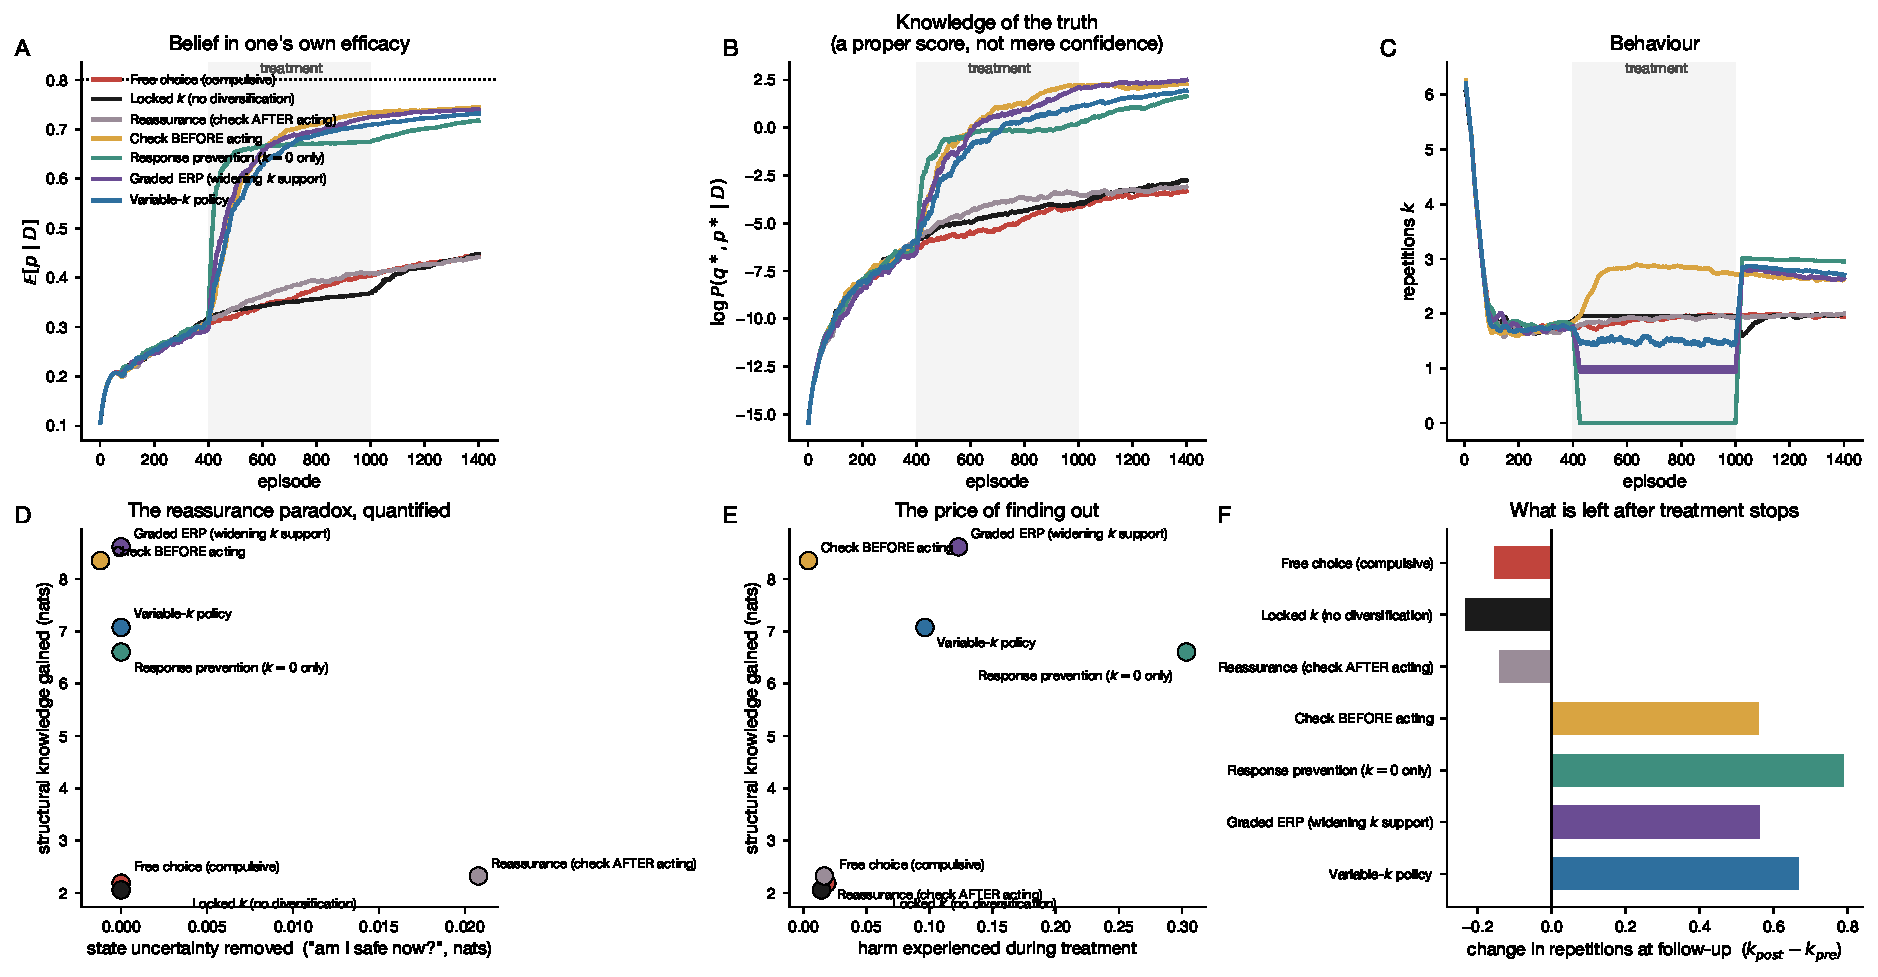
\includegraphics[width=\textwidth]{fig6_interventions.pdf}
\caption{\textbf{Interventions.} (A) Efficacy belief; the shaded band is the
treatment block. (B) Knowledge of the truth as a proper score. (C) Behaviour.
(D) The reassurance paradox: state uncertainty removed against structural
knowledge gained. (E) Knowledge gained against harm experienced. (F) Change in
repetition rate at follow-up: conditions that correct the agent's underestimate
of the baseline hazard raise it.}
\label{fig:fig6}
\end{figure}

\subsection{Where the trap lives, and what escapes it}

Sweeping the agent's initial belief about its own efficacy against the cost of
harm (Fig.~\ref{fig:fig4}) locates the trap. Initial doubt dominates: residual
error in the efficacy belief
falls from $\phaseHighDoubtErr$ for the most doubtful agents to
$\phaseLowDoubtErr$ for the most confident ($r = \phaseCorrDoubtErr$). The cost of
harm sets how much safety behaviour is performed ($r = \phaseCorrCostK$ against
$\log$ cost) but has no monotone relation to residual error once the agent acts
at all ($r = \phaseCorrCostErrHigh$ for costs above $6$).

What organises the whole diagram is the realised repetition count, and it does so
in the shape of a U (Fig.~\ref{fig:fig4}D). Agents that settle at $k=0$ --- those
for whom harm is cheap enough not to bother --- end $\phaseErrAtZeroK$ away from
the truth about their own efficacy, because $k=0$ is uninformative about $p$ by
Proposition~\ref{prop:two}; they pay for this with a harm rate of
$\phaseHarmAtZeroK\%$ and learn nothing from it. Agents that settle at
$k \approx \phaseBestK$ end $\phaseBestErr$ away, at a harm rate of
$\phaseHarmAtBestK\%$. Agents driven to $k \approx \phaseWorstHighK$ by a high
cost of harm end $\phaseErrHighK$ away, having experienced essentially no harm at
all. This is the same interior optimum found in the controlled design sweep
(Fig.~\ref{fig:fig3}F), now emerging from agents that were never told what to do:
never acting and always acting are both blind, and the cost of harm decides which
kind of blindness you get.

The information-seeking weight is the escape axis, and what it changes is
instructive. Among the most doubtful third of agents, residual error falls from
$\tauLoErrZero$ at $\tau=0$ to $\tauLoErrMax$ at $\tau=\tauMax$, and the efficacy
belief moves from $\tauLoMeanPZero$ to $\tauLoMeanPMax$ against a true $\worldP$.
What it changes to achieve this is worth being precise about, because it is not
what one might guess. The agent does not act much less
($\tauLoKZero$ repetitions against $\tauLoKMax$), and it does not visibly vary
more (variance of the action count $\tauLoVarZero$ against $\tauLoVarMax$). What
rises is the harm it actually experiences, from $\tauLoHarmZero\%$ of episodes to
$\tauLoHarmMax\%$. The escape is a shift towards repetition counts at which
outcomes still \emph{happen}, which is the same lesson the policy comparison in
Fig.~\ref{fig:fig2}D teaches: a ``compulsive but jittered'' policy on
$k \in \{5,6,7\}$ is formally non-singular and practically useless. Variation
buys nothing where nothing ever occurs.

Two caveats. The effect requires a substantial $\tau$: below about
$\tau \approx 45$ nothing moves, because the epistemic bonus is small next to the
cost of harm. And, as the hysteresis simulations make visible, the expected
information gain of an episode can be maximised at a \emph{large} $k$ when the
agent is pessimistic, so an information-seeking agent does not always explore
downward.

\begin{figure}[t]\centering
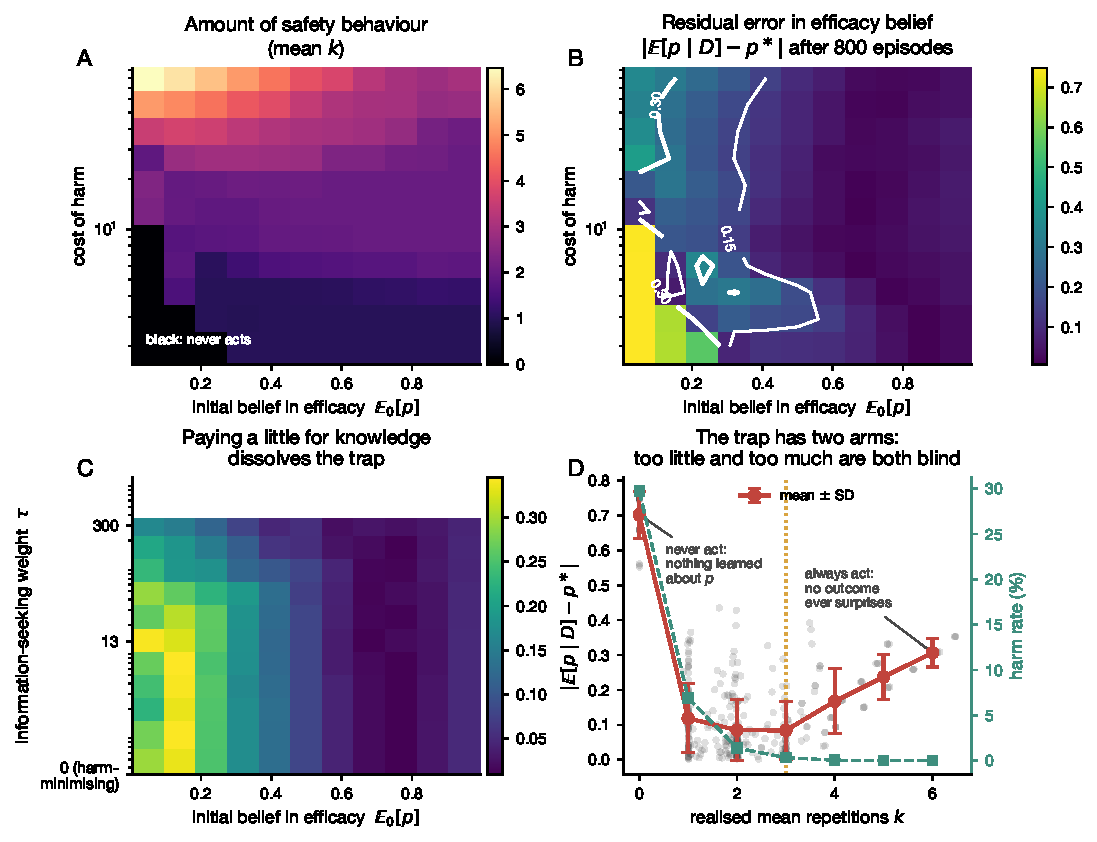
\includegraphics[width=\textwidth]{fig4_phase_diagram.pdf}
\caption{\textbf{Phase diagrams.} (A) Amount of safety behaviour and (B)
residual error in the efficacy belief over initial doubt and harm cost. (C) The
information-seeking weight as an escape axis. (D) Residual error against the
realised repetition count, pooled over the whole sweep: a U, with harm rate
(green, right axis) falling monotonically. Self-knowledge and safety are optimised
at different points.}
\label{fig:fig4}
\end{figure}

\subsection{Path dependence when the danger recedes}

Ramping the objective hazard up and back down (Fig.~\ref{fig:fig5}) produces
behavioural hysteresis in every arm, and we are careful about what that does and
does not show. Any belief-updating agent lags a moving world, so a loop by itself
is not diagnostic, and indeed the loop areas do not separate the arms
($\loopLocked$ for the locked design against $\loopQuota$ for an agent with a
standing $25\%$ response-prevention quota). What does separate them is
\emph{calibration}, and it does so asymmetrically. On the rising limb every arm
tracks the hazard about equally well ($|\mathbb{E}[q\mid D]-q| = \calibLocked$ up,
against $\calibQuota$ up). On the falling limb the locked design comes apart:
$\calibLockedDown$ against $\calibQuotaDown$ for the quota agent and
$\calibCheckerDown$ for an agent that checks. The trap is specifically a failure
to notice that the world has become safer, which is what the theory predicts: the
evidence that would carry that news is the evidence a repetitive policy suppresses.

Removing the hazard outright sharpens this into a single number. After the hazard
is set to zero, the locked agent takes $\stepLockedHalve$ episodes to halve its
repetition rate, still performs $\stepLockedK$ repetitions per episode at the end
of a $1500$-episode horizon, and believes the baseline hazard to be
$\stepLockedQ$ in a world where it is exactly zero. An agent with a standing
response-prevention quota takes $\stepQuotaHalve$ episodes and ends at
$\stepQuotaQ$; an information-seeking agent takes $\stepCuriousHalve$ --- five
times faster than the locked agent --- and ends at $\stepCuriousQ$.

The locked agent's terminal beliefs are worth reading carefully, because they show
the ridge doing its work. It ends convinced both that its actions are highly
effective ($\mathbb{E}[p\mid D] = \stepLockedP$) \emph{and} that the world remains
dangerous ($\stepLockedQ$) --- a pair that reproduces the harm rate it observes
(namely zero) exactly as well as the truth does, and that rationalises continuing
to act. Every arm that supplies a contrast converges instead on the correct low
hazard. This is the hysteresis prediction in its cleanest form: not that behaviour
lags, but that a policy which suppresses its own diagnostic evidence settles into
a self-confirming explanation of why it must continue.

\begin{figure}[t]\centering
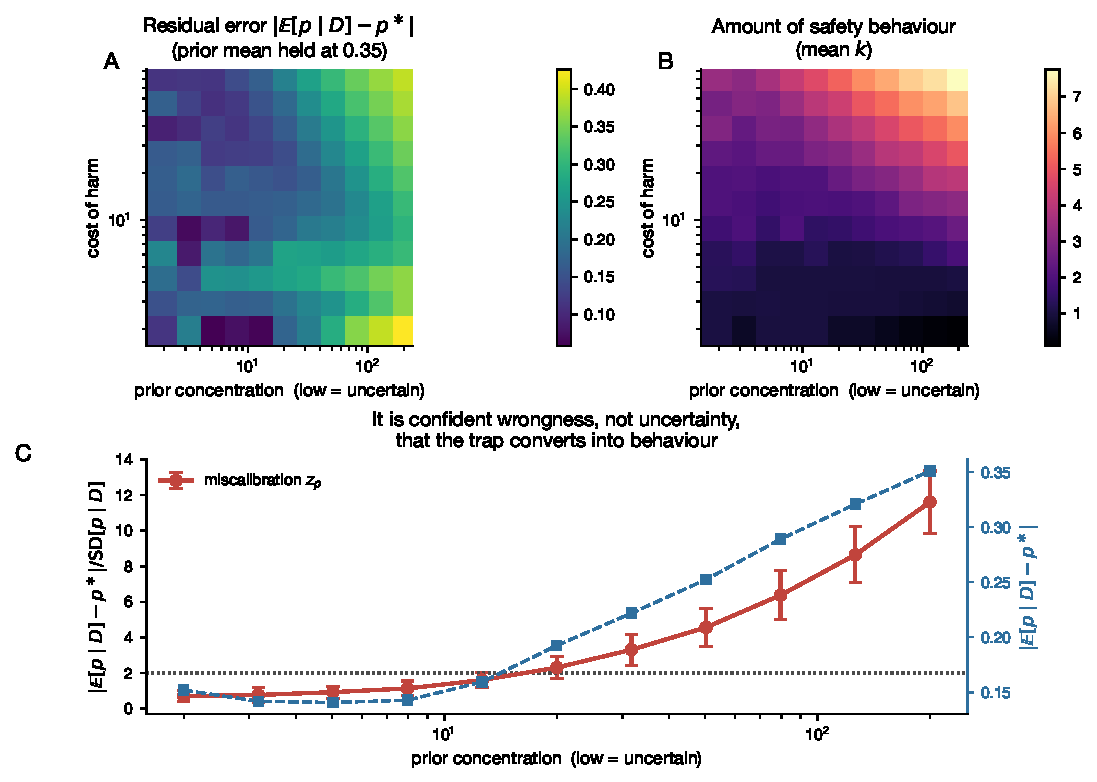
\includegraphics[width=\textwidth]{fig_S2_uncertainty_diagram.pdf}
\caption{\textbf{Supplementary: initial uncertainty against harm cost.} The prior
mean is held at $0.35$ throughout; only its concentration varies. (A) Residual
error, (B) amount of safety behaviour, (C) miscalibration and error against prior
concentration.}
\label{fig:figS2}
\end{figure}

\begin{figure}[t]\centering
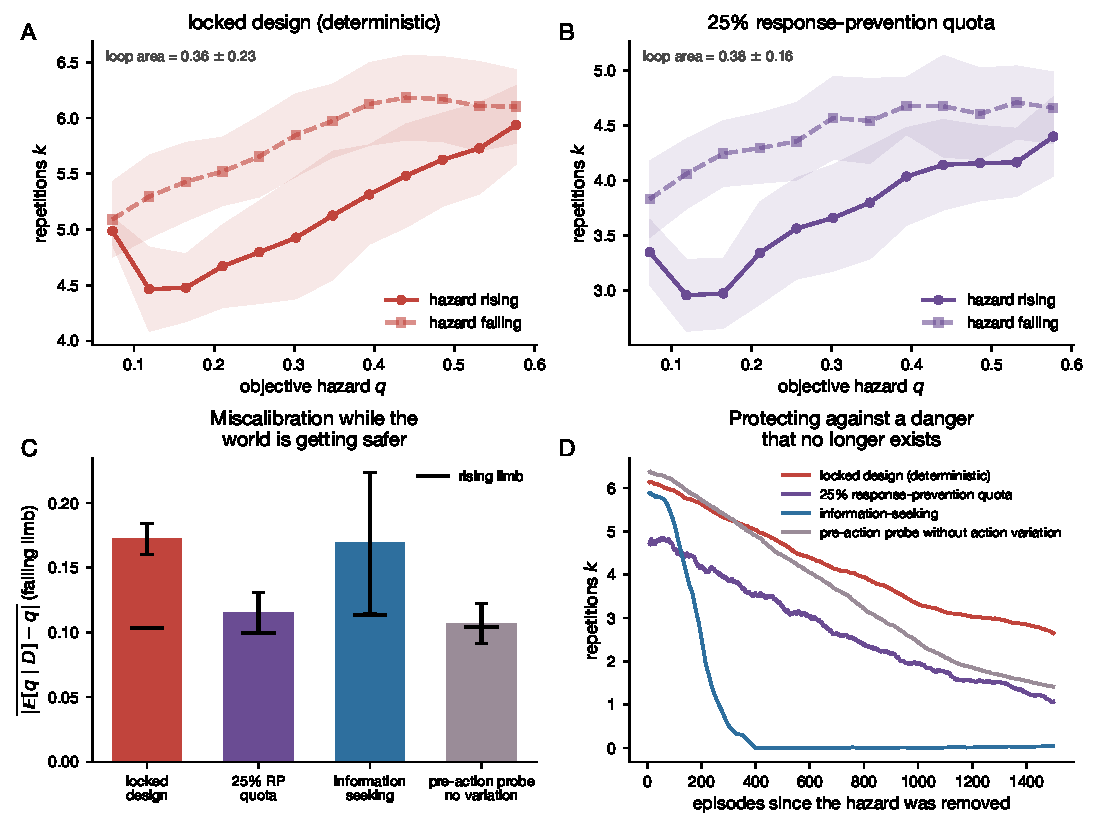
\includegraphics[width=\textwidth]{fig5_hysteresis.pdf}
\caption{\textbf{Path dependence.} (A,B) Repetition count against objective
hazard on the rising and falling limbs. (C) Belief miscalibration while the world
is getting safer. (D) Behaviour after the hazard is removed outright.}
\label{fig:fig5}
\end{figure}

\subsection{Predictions for human data}

The theory's distinctive empirical claim is not that compulsive people repeat
more. It is that, holding the amount of safety behaviour constant, its
\emph{variability} determines how much can be learned from it
(Fig.~\ref{fig:fig7}). Across designs matched exactly at $\mathbb{E}[k]=3$,
posterior uncertainty about efficacy falls from $\mathrm{SD}[p\mid D] =
\vmFixedSdP$ under a fixed design to $\vmBestSdP$ under the best varying one ---
a factor of $\vmSdRatio$ --- with
$\mathrm{corr}(\mathrm{Var}(k), \mathrm{SD}[p\mid D]) = \vmCorr$ across designs.
The price is visible too: harm rises from $\vmFixedHarm\%$ to $\vmBestHarm\%$ of
episodes. This is the cleanest prediction the model makes, because mean exposure
is matched by construction.

In a simulated population of $\popN$ individuals differing in initial doubt, cost
sensitivity and decision noise, we ask what predicts the \emph{accuracy} of the
efficacy belief that each individual ends up with. Where they started explains
much of it (adjusted $R^2 = \regBaseR$ from the initial belief alone). Adding how
much they acted and how much they varied adds nothing reliable
($p \regVarKP$ for $\mathrm{Var}(k)$) --- we report this because it is a real
null --- but adding the expected information their realised policy actually
generated raises the fit to $\regFullR$ ($p \regEigP$). What matters is not
variability as such but variability \emph{where outcomes still occur}, which is
what the information measure captures and a raw variance does not.

The non-circular form of the prediction is stratified. Decision noise inflates
both the mean and the variance of the action count, so an unstratified regression
of severity on $\mathrm{Var}(k)$ would be partly mechanical. Conditioning on
severity removes that path: within each of $\stratLevels$ strata of $\stratN$
individuals matched on how much safety behaviour they perform, individuals whose
behaviour varies more hold more precise beliefs about their own efficacy
(correlations between $\stratCorrMin$ and $\stratCorrMax$, negative in every
stratum).

Severity itself behaves as the theory predicts it should, with two separable
contributions. The initial efficacy belief alone explains almost none of it here
(adjusted $R^2 = \sevRegBase$, because the cost of harm dominates in this
population, reaching $\sevRegCost$ once cost is included); adding the
\emph{uncertainty} of the efficacy belief raises this to $\sevRegSdP$
($p \sevRegSdPP$) and adding policy-induced information raises it to
$\sevRegFull$ ($p \sevRegEigP$). Severity is predicted by how uncertain you are
and by how little your own behaviour tells you, not only by how low your estimate
is.

A direct human test would ask participants to choose how many preventive actions
to take before an outcome and fit this generative model. The predictions are
that (i) at matched mean exposure,
participants with higher trial-to-trial variability recover the true efficacy
parameter better; (ii) symptom severity is predicted by posterior uncertainty
about efficacy and by policy-induced information over and above the posterior
mean; and (iii) a reassurance-like probe reduces momentary confidence ratings
without improving efficacy estimates, while the same probe delivered before the
safety action improves both. If the posterior mean $\mathbb{E}[p]$ absorbs all
the variance, that would count against a contribution from policy-generated
information beyond belief bias.

\begin{figure}[t]\centering
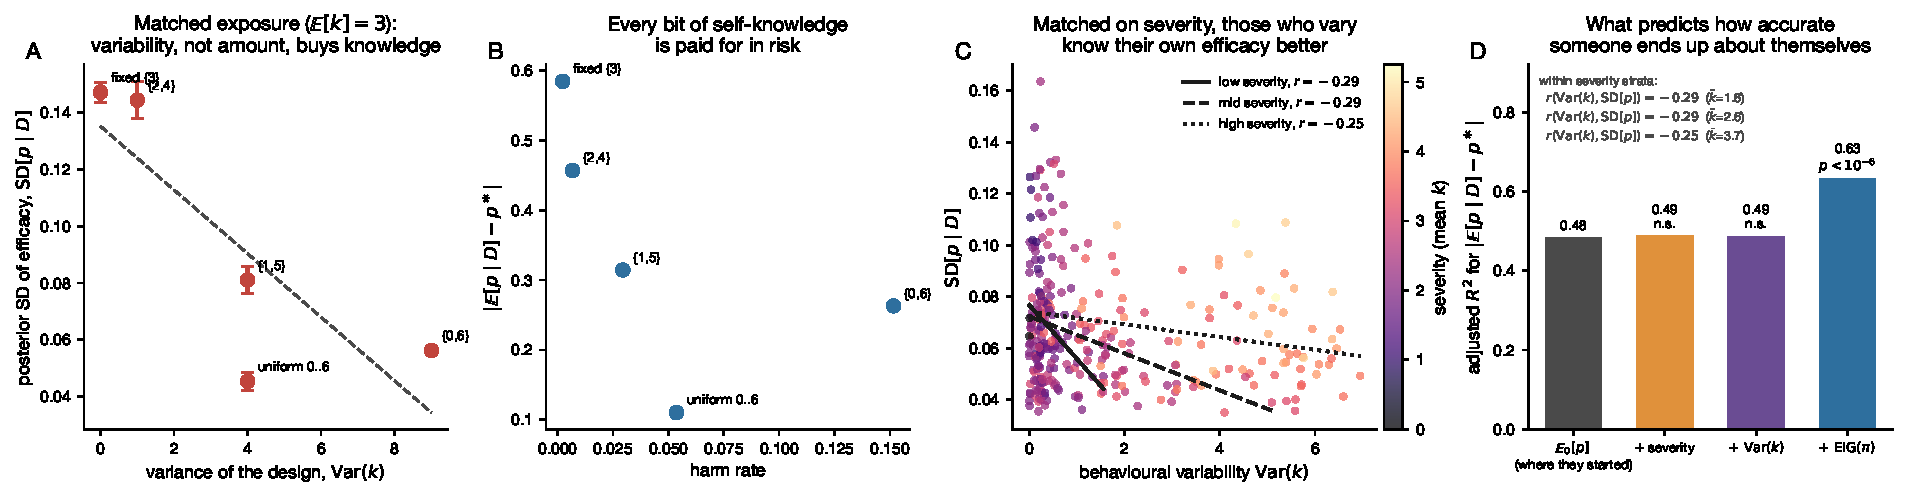
\includegraphics[width=\textwidth]{fig7_predictions.pdf}
\caption{\textbf{Falsifiable predictions.} (A) At matched mean exposure,
posterior precision about efficacy rises with the variance of the design.
(B) The price of that knowledge. (C) Simulated individuals. (D) Nested model
comparison for severity.}
\label{fig:fig7}
\end{figure}

\section{Discussion}

\subsection{Where this sits}

Table~\ref{tab:accounts} places the account among neighbouring proposals. The
claim is not that existing accounts are wrong; it is that policy-generated
non-identifiability is not explicitly represented in the cited accounts and
generates different predictions without assuming a learning deficit.

\begin{table}[t]\centering\small
\begin{tabular}{p{3.4cm}p{4.6cm}p{6.2cm}}
\toprule
\textbf{Account} & \textbf{Locus of pathology} & \textbf{Difference from the present account} \\
\midrule
\citet{rigoux2024beliefs} & A false point belief about preventive efficacy &
Here belief updating is exact; the policy makes the data non-identifying \\
\citet{fradkin2020latent} & Uncertainty about state transitions &
The transition learner need not be impaired \\
\citet{sakai2022eligibility} & Imbalanced eligibility traces &
Credit assignment is exact \\
\citet{gillan2014enhanced} & Habitual avoidance &
The effect precedes habitisation; information structure suffices \\
Repeated-checking literature & Degraded episodic memory confidence &
The uncertainty here is over latent causal parameters, not memories \\
Safety-behaviour literature & Safety behaviour blocks disconfirmation &
Formalised as rank deficiency in a specific pair of parameters \\
\bottomrule
\end{tabular}
\caption{The present account against its neighbours.}
\label{tab:accounts}
\end{table}

\subsection{Clinical implications}

\paragraph{Severity has two separable causes.} What predicts how much someone
repeats is not only how low their estimate of their own efficacy is, but how
uncertain that estimate is and how little information their own behaviour
generates. In the simulated population these are separable: the initial efficacy
belief alone explains adjusted $R^2 = \sevRegBase$ of severity, the uncertainty of
the efficacy belief raises this to $\sevRegSdP$, and policy-induced information
raises it to $\sevRegFull$. A person whose efficacy belief is mildly low but whose
policy is diverse recovers; a person with the same belief and a rigid policy does
not.

\paragraph{The trap need not look like excess.} Because the ridge admits two
readings --- ``the world is dangerous and I control it'' and ``the world is safe
and I do not'' --- a policy-induced rank deficiency can present as too much
protective behaviour or as too little. Our untreated agents drift towards the
second reading and end up acting less than the truth warrants while being
confidently wrong about the baseline hazard. If this transfers, it predicts a
subgroup whose problem is not visible as compulsion at all, and it cautions
against treating action frequency as the measure of the underlying disturbance.

\paragraph{Reassurance is not a weak version of exposure; it is a different
thing.} It reduces state uncertainty efficiently and structural uncertainty
hardly at all. This gives the well-known clinical observation --- reassurance
helps now and maintains the problem later --- a quantitative form, and it
suggests a concrete manipulation: in this model, the same checking behaviour,
performed \emph{before} rather than after the safety action, becomes diagnostic.
Whether this transfers to people remains an empirical question.

\paragraph{Response prevention should be understood as design, not as
extinction.} The dominant theory of exposure treats it as inhibitory learning
driven by expectancy violation \citep{craske2014inhibitory}. Our analysis is
compatible with that theory but says something more specific than ``exposure
works''.
Pure response prevention from a naive starting point is provably uninformative
about efficacy; it is the contrast between action counts that identifies. This
predicts that graded protocols which pass through several distinct levels of
safety behaviour should outperform protocols that jump to zero and stay there.
In our simulations the jump-to-zero protocol still works, because the patient's
own repetitive history supplies the other half of the contrast --- but it works
for a reason that a naive reading of exposure would not predict, and it fails
outright in the one condition where that history is absent.

\subsection{Knowing that you are in control}

There is a philosophical claim buried in the mathematics. To know that you
control something, it is not enough to observe that things go well when you act.
You must have varied what you do and compared. Knowledge of one's own agency is
not available by introspection; it depends on counterfactual access, and
counterfactual access is something a policy can destroy. The literature on the
sense of agency has largely studied the subjective experience of control
\citep{haggard2017sense,moore2016agency,gentsch2012agency};
the present account concerns a level above that --- not the feeling of control but
knowledge of controllability, and the conditions under which such knowledge is
obtainable at all. It is a special case of a general point in causal learning:
identifying a causal structure requires choosing informative interventions, not
merely observing outcomes \citep{he2008active}. What is distinctive about the
clinical case is that the agent choosing the interventions is the same agent whose
own efficacy is the parameter in question, and that the intervention it most wants
to make is the one that tells it least.

Philosophically, the picture also inverts a familiar description of the disorder.
\citet{dehaan2015} argue that people with obsessive-compulsive disorder become
free by losing control --- that relinquishing the attempt at control is what
restores agency. The present model gives that a formal reading: releasing the grip
on the action is precisely what restores the variation from which controllability
can be inferred.

\subsection{The same structure elsewhere}

The trap is not specific to compulsion. In system identification, a controller
that regulates a plant too well stops exciting it and loses the ability to
identify it. In economics, self-confirming equilibrium describes beliefs about
off-path contingencies that survive because those contingencies are never visited
\citep{fudenberg1993selfconfirming}. In machine learning, the selective labels
problem describes outcomes that are observable only for the cases past decisions
selected \citep{lakkaraju2017selective}, and algorithmic feedback loops describe
policies that generate their own future training data
\citep{chaney2018algorithmic}. Safe reinforcement learning confronts the same
trade-off directly: learning an unknown dynamics requires exploration, and
exploration is exactly what a safety constraint forbids
\citep{moldovan2012safe}. Overuse of diagnostic testing in defensive medicine may
have the same shape, though we offer this as an analogy to be tested rather than
a result.

Stated generally: \emph{safety-seeking creates a tension between control and
knowledge. To learn whether an intervention works, an agent needs variation in
the intervention and access to outcomes under alternatives. When the cost of
failure is high, short-term optimal behaviour suppresses exactly that variation.}
Compulsions may be one instance of a broad class of epistemic traps in which the
policy chosen to control uncertainty also determines, and impoverishes, the
evidence available for resolving it.

\subsection{Limitations}

The clearest limitation is one the results themselves force. Within the horizons
we simulate, the trap is reliably \emph{epistemic} --- the agent's model of itself
and its world stays wrong, and stays wrong with unwarranted confidence --- but it
is not reliably \emph{behavioural}: a purely harm-minimising agent's repetition
count decays even while its beliefs do not recover, and adding uncertainty
aversion strengthens the loop without closing it. A complete account of persistent
compulsive \emph{behaviour} therefore needs at least one ingredient this model
does not contain. What the model does supply is an explanation of why the belief
never gets corrected, which is the part the existing accounts leave open.

The hazard model is a deliberate reduction of the Rigoux scenario and omits
within-episode sequential decision making: our agent commits to $k$ before the
episode rather than choosing repetition by repetition. The environment is
stationary except where explicitly ramped, and the agent has no model of change,
so its ability to track a moving hazard depends on an exponential forgetting
factor rather than on a change-point model. Harm is observed without noise, which
is generous to the agent; observation noise would not restore identification and
would generally reduce information. Our
interventions are idealised: a real ERP protocol changes many things at once, and
we have isolated one of them. Finally, no human data are analysed here; the
account stands or falls on the predictions in Section~3.8, and we have tried to
state them in a form that can fail.

\section*{Data and code availability}

All simulations are grid-based and deterministic given a seed. The complete
source code, result tables, figure-generation scripts and manuscript sources
will be released in a public repository before submission; the repository URL
and an archival DOI will be added here before upload. Every number in this
manuscript is generated into \texttt{paper/numbers.tex} directly from the saved
result files, so the prose cannot drift away from the data.

\bibliography{references}

\end{document}
